\subsection{updating chunks}
Terrain modification consists of two main steps:
\begin{enumerate}
    \item the scalar field for the modified chunk has to be altered, which involves iterating over a 3-dimensional array of numbers and modifying the values stored in that array using some function,
    \item a new mesh has to be generated based on the new values of the scalar field.
\end{enumerate}
Since the modifications happen 60 times a second and the number of operations they require is rather big (of the order of the chunk size, i.e. $16^3$) it's unfeasible to do them on the main thread without severe lags.
Thus most of the work related to terrain modification is delegated to the worker thread.

The workflow for terrain modification can be described as follows.
The main thread in the \texttt{Pickaxe.ModifyTerrain} method determines which chunks are going to be affected by the terrain modification, and adds them to a buffer \texttt{buffer}.
Once all the chunks are in \texttt{buffer}, we set the \texttt{IsProcessingBatch} flag to \texttt{true} (while set to true, no further terrain modifications will be registered) and enqueue each of them into the \texttt{modificationsToPerform} queue along with some additional information (passed in the form of an instance of \texttt{ModificationArgs} struct) necessary to perform the modification.
A very important piece of information is the \texttt{batchSize} which is the size of \texttt{buffer} (its importance will become apparent later).

The worker thread dequeues chunks from the \texttt{modificationsToPerform} queue.
It modifies the scalar field using the information passed in \texttt{ModificationArgs} and generates a new mesh based on the scalar field.
Once new vertices for the mesh are calculated, it enqueues the chunk together with \texttt{batchSize} (retrieved from \texttt{modificationArgs}) into the \texttt{updatedChunks} queue.

In the \texttt{ResolveUpdated} function the main thread dequeues the \texttt{(chunk, batchSize)} pair from the \texttt{updatedChunks} queue and adds \texttt{chunk} to the \texttt{currentBatch} list.
Once the number of chunks in \texttt{currentBatch} is equal to \texttt{batchSize} of the dequeued chunk, it means that the main thread has "received back" all of the chunks from a single modification call.
The main thread then updates the GPU buffers with the new vertices of the chunk's mesh and updates the shape of the collision surface in the physics engine for each chunk from \texttt{currentBatch}.
Once the whole \texttt{currentBatch} is updated, the \texttt{IsProcessingBatch} flag is set back to false.

The whole process is depicted in \autoref{fig:chunk-worker}.
\begin{figure}[h] % https://drive.google.com/file/d/1TzJouYAys_fz1GkhppZsqoh9yFn62twL/view?usp=sharing
    \centering
    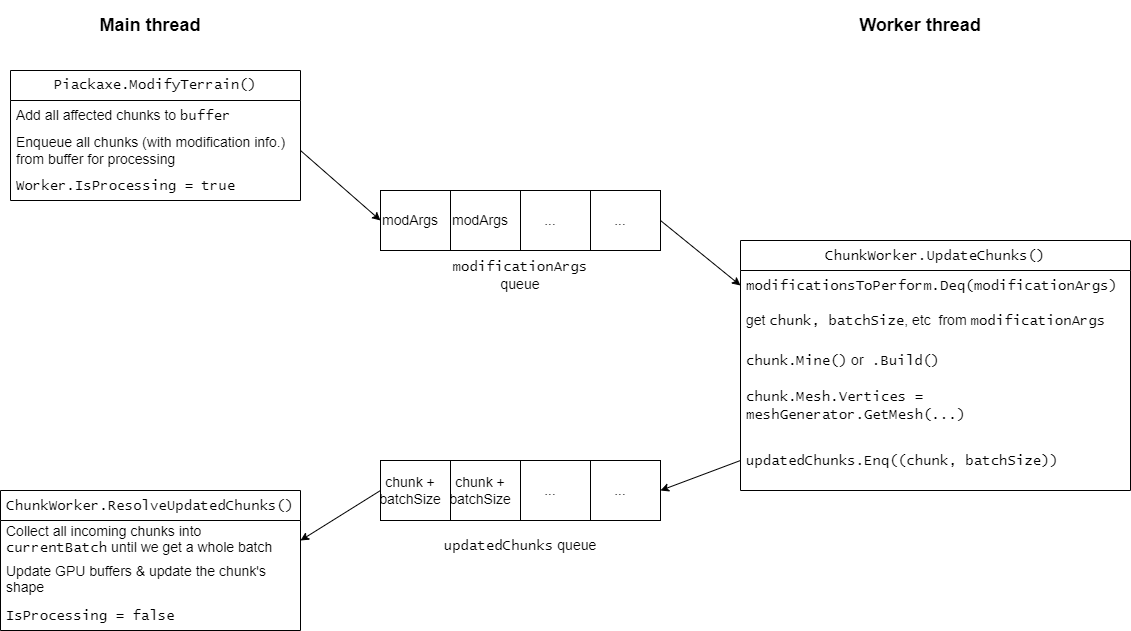
\includegraphics[width=1\textwidth]{chapters/system_architecture/sections/chunk_worker/resources/chunkWorker.drawio.png}
    \caption{Terrain modification in the chunk management system}
    \label{fig:chunk-worker}
\end{figure}

The reason for processing chunks in batches rather than individually is simple.
If we modify chunks one by one it may be the case that when the terrain is rendered, one chunk has already been modified, while its neighbor has not, resulting in a visible gap between the two.
This problem can be seen in \autoref{fig:gaps-between-chunks-chunk-worker} which comes from an early stage of the game's development.
\begin{figure}[h]
    \centering
    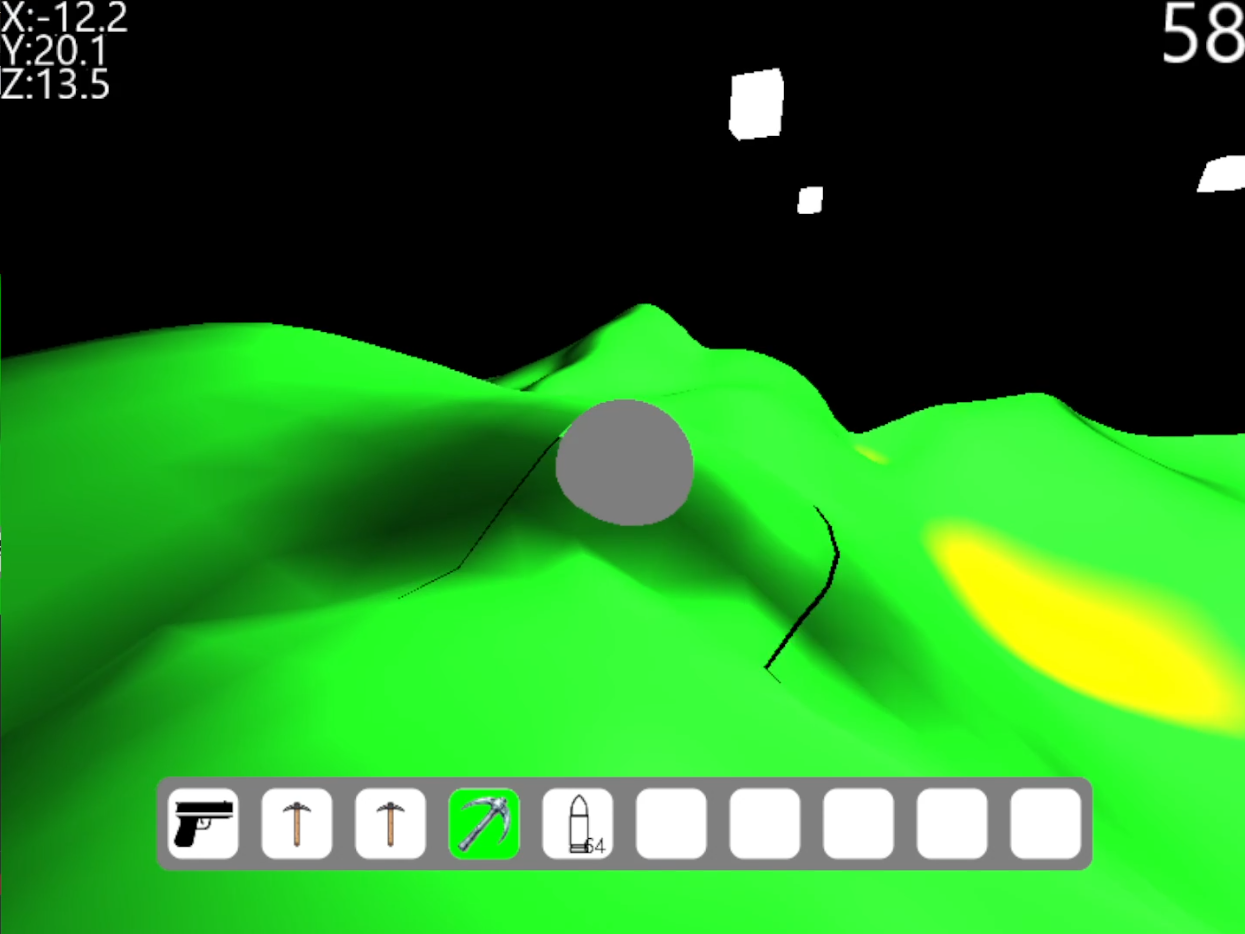
\includegraphics[width=0.8\textwidth]{chapters/system_architecture/sections/chunk_worker/resources/gaps-between-chunks.png}
    \caption{Gaps between chunks appearing during terrain modification}
    \label{fig:gaps-between-chunks-chunk-worker}
\end{figure}

One drawback of this approach is that the main thread doesn't register new chunks for modification while the whole previously enqueued batch hasn't been processed.
This could cause the modification rate to be irregular should the main thread "drop" a lot of modifications.
To deal with this problem, the modification depends on the time elapsed between two modifications.